\documentclass{article}
\usepackage[frenchb]{babel}
\usepackage{amsfonts}
\usepackage{amsmath}
\usepackage[T1]{fontenc}
\usepackage[utf8]{inputenc}
\usepackage{amsthm}
\usepackage{graphicx}
\usepackage{tikz}
\usepackage{tikz-cd}
\usepackage{hyperref}

\hypersetup{                    % parametrage des hyperliens
    colorlinks=true,                % colorise les liens
    breaklinks=true,                % permet les retours à la ligne pour les liens trop longs
    urlcolor= blue,                 % couleur des hyperliens
    linkcolor= blue,                % couleur des liens internes aux documents (index, figures, tableaux, equations,...)
    citecolor= cyan               % couleur des liens vers les references bibliographiques
    }

\title{Histoires gaussiennes }
\date{}
\author{ Clément Dell'Aiera}


\newtheorem{definition}{Definition}
\newtheorem{thm}{Théorème}
\newtheorem{ex}{Exercice}
\newtheorem{lem}{Lemme}
\newtheorem{dem}{Preuve}
\newtheorem{prop}{Proposition}
\newtheorem{cor}{Corollaire}

\newcommand{\Z}{\mathbb Z}
\newcommand{\R}{\mathbb R}
\newcommand{\C}{\mathbb C}
\newcommand{\Hil}{\mathcal H}
\newcommand{\Mn}{\mathcal M _n (\mathbb C)}
\newcommand{\K}{\mathbb K}
\newcommand{\B}{\mathbb B}
\newcommand{\Cat}{\mathbb B / \mathbb K}

\begin{document}
\maketitle

\begin{figure}[!h]\centering
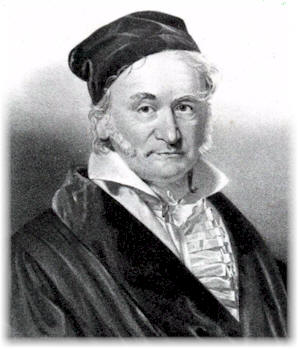
\includegraphics[scale=0.4]{Gauss2.jpg}
\caption{Gauss}
\label{fig:Gauss2}
\end{figure}

\newpage
\tableofcontents

\newpage

%\section{Problèmes antiques}
%Quadrature du cercle
%Duplication du cube
%Trisection de l'angle
%%%%%%%%%%%%%%%%%%%%%%%%%%%%%%%%%%%%%%%%%%%%%%%%%%%%%%%%%%%%%%%%%%%%%%%%%%%%%%%%%%%%%%%%%
%%%%%%%%%%%%%%%%%%%%%%%%%%%%%%%%%%%%%%%%%%%%%%%%%%%%%%%%%%%%%%%%%%%%%%%%%%%%%%%%%%%%%%%%%

%FAIRE UNE INTRO ET UNE CONCLUSION
\begin{abstract}
Ce rapport s'intéresse aux origines de la loi normale. Nous étudierons comment, à partir d'une méthode empirique, est née la méthode des moindres carrés, qui a fourni le cadre théorique adéquat pour l'émergence d'un <<postulat gaussien>> en ce qui concerne la loi des erreurs. Ce postulat, remis en cause à partir des travaux de Paul Lévy, est une des origines du modèle de Bachelier-Osbourne en finance, et d'une grande partie de l'ingénieurie financière actuelle. Nous terminerons par l'analyse de paradigme gaussien et de son impact sur les théories économique, et son lien avec le concept d'efficience de marché. En particulier, nous essaierons de mettre en évidence une controverse sur ce point.
\end{abstract}
\section{Problèmes du début du XIX siècle}

L'heuristique qui va mener à la méthodes des moindres carrés débute avec un problème simple : résoudre un système d'équations linéaires surdéterminé, c'est-à-dire que le nombre d'équations surpasse le nombre d'inconnues. De façon générale, un tel système n'a pas de solution. Pourtant, lorsque les astronomes travaillent à determiner les positions des corps célestes, ils effecuent de nombreuses mesures, dont les erreurs empêchent une solution exacte.\\

Notre histoire commence un peu avant $1800$, et met en scène des navigateurs, des cartographes et des astronomes. Tous sont concernés par le futur concept \textit{d'erreur de mesure}. Rappelons que la physique de l'époque est marquée par l'oeuvre de Newton, qui a publié en $1686$ son célèbre ouvrage \textit{Philosophiae Naturalis Principia Mahtematica}. Son oeuvre permet aux scientifiques de déterminer des grandeurs innaccessibles à l'observation, telles que la constante de gravitation $\mathcal G$. \\

A posteriori, on peut même déjà détecter les prémisses du \textit{primat euclidien} qui imprègne l'époque des Lumières dans sa réduction de la mécanique du solide à celle du point. La mécanique de Newton décrit le mouvement d'un solide par celui de son centre de gravité, qui est le point dudit solide qui minimise la fonctionnelle $x\mapsto \int_S ||Mx||^2 \mu(dx)$, où $S$ représente le solide, et $\mu$ sa distribution de masse. On verra qu'il y a bien un lien entre la méthode des moindres carrés et la minimisation d'une certaine norme euclidienne (la somme des carrés des erreurs).\\ 

De manière générale, les systèmes linéaires que doivent résoudre les astronomes, par exemple pour déterminer les constantes, sont surdeterminés, au sens où il y a plus d'équations que d'inconnues. Ils ne possèdent donc pas en général de solution. En effet, un système surdeterminé qui possèderait une solution doit nécessairement posséder plusieurs équations proportionnelles. Or la moindre perturbation, un erreur de mesure par exemple, empêche cela. La prochaine section présente un petit interlude qui reprend, avec une formulation moderne, ce problème de surdétermination avec l'exemple du <<point d'intersection>> de trois droites non concourantes. Il est à noter que c'est cette approche qui ménera les géomètres à imaginer des espaces de dimension supérieure à $3$. Trouver le point de Lemoine revient en effet à se placer en dimension $3$ à partir du triangle (qui vit en dimension $2$), pour ensuite projeter un certain point sur ce plan. La généralisation en dimension $3$, trouver le point qui minimise la somme des distances au carrées des faces d'un tetraèdre, peut se résoudre en considérant le projeté d'un point en dimension $4$. Bien que les calculs fonctionnaient très bien et donnaient la bonne solution, le pas conceptuel à été d'une difficulté considérable : les espaces de la géométrie pouvaient-ils s'affranchir de l'espace <<réel>> à $3$ dimensions ? Même un mathématicien aussi audacieux que Henri Poincaré répugnera lontemps à utiliser des dimensions supérierues à $3$.

\subsection{Point de Lemoine}
 Pour simplifier le problème et illustrer de manière simple notre propos, plaçons nous dans le plan, et choisissons trois droites au hasard. La situation générique est alors celle de droites non concourantes, s'intersectant deux à deux. Le problème considéré revient alors à se poser la question suivante : quel est le point d'intersection de ces droites ? Au sens strict bien sûr, il n'existe pas. Pourtant, on peut sûrement décréter qu'un certain point est le meilleur candidat. Lequel ?\\

Le partisan du primat euclidien voudra naturellement ici minimiser la somme des carrés des distances au droites : le meilleur point est celui, $M$, dont la somme 
  \[d(M,D_1)^2+d(M,D_2)^2+d(M,D_3)^2\]
est minimale.\\

Nous pouvons repérer $M$ par ses coordonnées barycentriques liées au triangle formé par les trois points d'intersection $A_{j}$ des trois droites $D_j$, $j\in\{1,2,3\}$ : 
\[M=(\mathcal A_1,\mathcal A_2,\mathcal A_3)\]
où $\mathcal A_j$ est l'aire du triangle formé par $M$ et les $2$ points opposés à $A_j$. L'aire $\mathcal A_j$ est proportionnelle à la hauteur $h_j$ de ce triangle, i.e. à a distance de $M$ à $D_j$. Minimiser la somme des carrés des distances aux trois droites revient donc à minimiser 
\[h_1^2+h_2^2+h_3^2\quad s.c.\quad ah_1+bh_2+ch_3=2s\]
où $a$, $b$ et $c$ sont respectivement les longueurs des côtés $A_2A_3$, $A_1A_3$ et $A_1A_2$. Le principe des extremas liés donne la solution :
\[M=(a^2,b^2,c^2)\]
Si le triangle est équilatéral, la remarque suivante permet d'y voir plus clair : la somme des carrés d'un triplet dont la somme est fixée est atteinte pour le triplet équiréparti. Voir la figure \ref{Lemoine}. Pour plus de détails sur la géométrie classique, le lecteur peut se reporter à l'ouvrage de Jean-Denis Eiden. ~\cite{Eiden} \\

\begin{figure}[!h]\centering
\begin{tikzpicture}[scale = 3]
\draw (0,0) -- (1,1);
\draw (0,0) -- (2,0);
\draw (1,1) -- (2,0);
\fill[gray] (0,0) -- (1,1) -- (1,0.5) -- cycle;
\draw[dashed] (1,0.5) -- (2,0);
\draw[dashed] (1,0.5) -- (0,0);
\draw[dashed] (1,0.5) -- (1,1);
\draw (0.75,0.6) node{$\mathcal A_3$};
\draw (0,0) node[left]{$A_1$} ;
\draw (2,0)  node[right]{$A_3$};
\draw (1,1)  node[above]{$A_2$};
\draw (1,0.5) node{$\times$};
\draw (1,0.5) node[right]{$M$};
\end{tikzpicture}
\caption{\textbf{Point de Lemoine.} L'aire grisée est proportionnelle à la coordonnée barycentrique de $M$ relative à $A_3$.}
\label{Lemoine}
\end{figure}


\subsection{Quatre problèmes}
 
Quatre problèmes vont en particulier contribuer au dévelopement de la méthode des moindres carrés. La libration de la Lune, les inégalités de mouvement de Jupiter et Saturne, la stabilité du sysème solaire, et la forme de la Terre. \\

Le problème de la libration de la Lune vient de celui de la détermination de sa postion sur le globe. Les marins se repèrent en effet grâce à de savants calculs astronomiques. Par exemple, déterminer sa longitude est facile. Celle-ci est l'angle entre la normale au point considéré et la normale à l'équateur, c'est-à-dire approximativement celui entre l'horizon et un point à l'infini (l'étoile polaire par exemple \label{ellipse}), facile à determiner à l'aide d'un sextant. Par contre, la longitude est difficile à obtenir. Si vous disposez d'une très bonne horloge et de l'heure du point auquel vous vous trouvez, vous pourriez le faire : il suffit pour cela de régler l'heure de l'horloge sur celle d'un méridien de référence, et de comparer la différence d'avec votre heure. Mais les horloges de l'époque ne permettent pas ce genre de technique... \\

Tobias Mayer propose en$1749$ de se servir des mouvements de la Lune pour determiner sa longitude. En effet, bien que la Lune nous présente toujours la même face, elle ne nous la présente pas toujours de la même façon. La variation de son axe de rotation par rapport au plan de rotation de la Terre fait que, sur un temps long, la Lune expose environ $60\%$ de sa surface à l'oeil terrestre. En se basant sur une relation compliquée entre plusieurs points de référence, Tobias Mayer parvient à proposer une méthode de localisation. Pour plus de détails, nous renvoyons à l'ouvrage de Stigler.~\cite{Stigler} L'important est que T. Mayer se doit de déterminer certaines constantes expérimentales de sa relation, et que pour cela il des observations du cratère Manilius, afin d'augmenter la précision de ce que l'on appellerait aujourd'hui des estimateurs.\\ 

Les inégalités du mouvement de Saturne et Jupiter s'attaque à une inadéquation entre les mouvements théoriques que prévoit la théorie de la gravitation de Newton, et ceux observés. Il convient de rappeler que les mouvements des planètes sont en première approximation donnés par leur seule interaction avec le Soleil. Les interactions avec les autres planètes sont jugées négligeables en raison de leur masse, bien plus faible que celle d'une étoile. Cette approximation permet de calculer effectivement les orbites des planètes, puisque l'on se sait pas résoudre explicitement les équations du mouvement pour $3$ corps. Et pourtant, les géantes Jupiter et Saturne ne semblent pas se plier à cette approximation. L'Académie des Sciences propose alors un concours pour expliquer ce phénomène, concours que Euler remportera avec son mémoire \textit{Recherches sur les inégalités du mouvement de Jupiter et Saturne}. Dans ce mémoire, après avoir effectuer une analyse mathématique, Euler essaie de vérifier sa méthode au moyen de mesures expérimentales. Il utilise, comme Mayer, une méthode de régroupement des observations, mais n'arrive pas à conclure. Pour plus de détails, nous renvoyons toujours à l'ouvrage de Stigler. ~\cite{Stigler}\\

Mayer et Euler aboutissent donc à une méthode de regroupement des observations. Euler échoue, peut-être à cause de son manque pratique expérimentale. Laplace rependra ce problème, et propose la méthode des moindres carrés, mais en norme $L1$ : avec une intuition folle, il donne en substance la méthodologie des MCO mais ne parvient pas à un résultat satisfaisant. C'est une constante chez Laplace, comme on le verra. Il aura souvent la bonne intuition, mais se trompera légèrement et n'arrivera pas à aboutir. Ici, son <<erreur>> a été de vouloir minimiser la somme des valeurs absolues des erreurs, et non leur carré.\\

Legendre y arrive d'une façon aboutie, mais sans modélisation probabiliste, ce qui l'empêche de quantifier l'erreur faite par MCO.  A partir du travail de Legendre, les MCO, bien qu'assise théoriquement, mettront plus de $50$ ans à s'imposer, la méthode de Mayer restant la préférée des praticiens. Gauss puis Laplace fonde la méthode sur une base solide.\\
%FINIR

%\subsection{Forme de la Terre}
Présentons le dernier problème. A partir de Newton, l'idée que la Terre n'est pas exactement une sphère a fait son chemin, et la détermination de sa forme devient l'un des problèmes scientifiques de premier plan. La théorie newtonienne de la gravitation prévoit qu'elle soit aplatie aux pôles, mais les Français, menés par l'astronome Cassini, pensent eux qu'elle l'est à l'équateur. Pour trancher, différentes équipes décident d'organiser des expéditions afin de mesurer la courbure du globe à différents endroits éloignés. Pour cela est décidée la procédure suivante : on va mesurer la distance entre les latitudes, c'est-à-dire la longueur d'un arc joignant deux points de même longitude situés à deux latitudes différentes. \\

Les astronomes supposent que la Terre a une forme d'ellipse lorqu'on la coupe selon un plan vertical. Rappelons que la latitude est paramétrée par l'angle que fait la normale par rapport au plan de l'équateur, aussi la distance entre deux latitudes est plus grande aux pôles qu'à l'équateur. Notre brave ellipse d'équation :
\[\left(\frac{x}{a}\right)^2+\left(\frac{y}{b}\right)^2=1\]
peut être paramétrée par $\theta$ :

\[\left\{\begin{array}{c} a\cos\theta \\ b \sin\theta \end{array}\right.\]

\[T_\theta=\left\{\begin{array}{c}-a\sin\theta \\ b\cos\theta\end{array}\right.\quad N_\theta=\left\{\begin{array}{c}b\cos\theta \\ a\sin\theta\end{array}\right.\]
La latitude $\phi$ verifie alors :
\[\left\{\begin{array}{c}
\cos\phi=\frac{b\cos\theta}{\sqrt{b\cos \theta+a\sin\theta}}\\
\sin\phi=\frac{a\sin\theta}{\sqrt{b\cos \theta+a\sin\theta}}
\end{array}\right.\]
 A partir de ces formules furent estimées des longueurs d'arc à différents points du globe. C'est Boscovich qui, le premier, publie dans \textit{De Litteraria Expeditione per Pontificiam ditionem ad dimetiendas duas Meridiani gradus}, une méthode pour traiter des mesures non concordantes. \\

\begin{figure}[!h]\centering
\begin{tikzpicture}[scale = 3]
\draw (0,0) ellipse (1.3 and 1);
\draw (0,0) node{$\times$};
\draw (0,0) node[above left]{$C$};
\draw[->] (0,-1.3) -- (0,1.3);
\draw[->] (-1.5,0) -- (1.5,0);

\draw (1.3*0.866,0.5) node[below left]{$M$};

\draw[blue,->] (1.3*0.866,0.5) -- ++ (0.5*0.866,0.5*1.3*0.5);
\draw[blue] (1.3*0.866,1.3*0.5) node[above right]{$N_\phi$};
\draw[blue,->] (1.3*0.866,0.5) -- ++ (0.5,0);
\draw[->] (1.3*0.866+0.25,0.5) arc (0:30:0.25);
\draw (1.3*0.866+0.25,0.5) node[above right]{$\phi$};

\draw[dashed] (1.3*0.866,0.5)-- ++ (0.5*1.3*0.5,-0.5*0.866);
\draw[dashed] (1.3*0.866,0.5)-- ++ (-0.5*1.3*0.5,0.5*0.866);
\draw (1.3*0.866-0.05*1.3*0.5,0.5+0.05*0.866) -- ++ (0.05*0.866,0.05*1.3*0.5) -- ++ (0.05*1.3*0.5,-0.05*0.866) ;
\end{tikzpicture}
\caption{\textbf{Forme de la Terre.} La latitude $\phi$ est donnée par l'angle entre la normale avec le plan de l'ecliptique. }
\label{Ellipse}
\end{figure}

L'aboutissement statistique de ces $4$ problèmes sera la publication par Legendre en 1805 de la méthode moderne des moindres carrés dans son supplément à l'article \textit{Nouvelles méthodes pour la détermination des orbites des comètes}. Son exposition est très claire et ressemble fort à ce que l'on pourrait trouver dans les livres actuels.\\

%%%%%%%%%%%%%%%%%%%%%%%%%%%%%%%%%%%%%%%%%%%%%%%%%%%%%%%%%%%%%%%%%%%%%%%%%%%%%%%%%%%%%%%%
%%%%%%%%%%%%%%%%%%%%%%%%%%%%%%%%%%%%%%%%%%%%%%%%%%%%%%%%%%%%%%%%%%%%%%%%%%%%%%%%%%%%%%%%
\section{La synthèse Gauss-Laplace}

\subsection{D'une méthode empirique}

Au milieu du XVIIIe siècle, une recette empirique est utilisée pour, face à plusieurs mesures d'un même paramètre, en donner la valeur "la plus probable" : c'est la méthode du milieu. Sa provenance est floue : plusieurs auteurs pensent que les marins, lorsqu'ils prennaient des mesures astronomiques afin de déterminer leur position sur le globe, gardaient naturellement le milieu entre deux mesures, puis en sont venus à l'idée de moyenne arithmétique.\\

La première apparition publiée (à titre posthume en 1722) de cette méthode date d'un texte de Cotes, ce qui lui a valu l'appellation de règle de Cotes :\\

\begin{quotation}Let p be the place of some object defined by observation, q,r,s the places of the same object from subsequent observations. Let there also be the weights P, Q, R, S reciprocally proportional to the displacements which may arise from the errors in the single observations, and which are given from the given limits of error; and the weight P, Q, R, S are conceived as being placed at p,q,r,s and their center of gravity Z is found : I say the point Z is the most probable place of the object, and may be the most safely had for its true place. (Cotes, 1722, p.22; based on the translation by Gowing, 1983, p.107)\end{quotation}

L'intérêt de la citation réside pour moi dans le fait suivant : cette méthode est loin d'être claire ! De façon générale, lorsque l'on se réfère à l'époque à cette règle, c'est de façon totalement empirique : les conseils pour appliquer la méthode sont farfelus, même s'ils constituent finalement la base d'un futur procédé statistique. Par exemple, les auteurs conseillent de ne l'appliquer qu'à des mesures faites par un seul observateur, dans des conditions semblables et pas trop éloignées dans le temps.

\subsection{Méthode des moindres carrés}

L'astronome Piazzi, le $1$er janvier $1801$, observe un corps célestes d'un diamètre cinq fois inférieur à celui de la Lune pendant moins de $3$ minutes d'arc, puis le perd de vue le $11$ février de la même année, sans qu'aucun astronome ne puissent le localiser à nouveau.\\

Il s'agit du premier astéroïde observé, Cérès. Le $7$ décembre $1801$, von Zach le retrouve à l'emplacement indiqué par Gauss, qui ne publie ses calculs ni ne donne sa méthode avant $1809$ dans son article \textit{Théorie du mouvement des corps célestes}. Il utilise la méthode des moindres carrés, déjà développée par Legendre dans son supplément à l'article \textit{Nouvelles méthodes pour la détermination des orbites des comètes} de $1805$. Bien sûr, Gauss ne mentionne pas les travaux de Legendre, et ne paraît pas en avoir eu connaissance. Comme preuve, il avance son calcul de l'orbite de Cérès $4$ ans avant la publication de Legendre et écrit :
\begin{quotation}
"Au reste, ce principe dont nous avons fait usage dès l'année $1795$ a été donné dernièrement par Legendre dans ses Nouvelles Méthodes..." (Gauss, Théorie du mouvement des corps célestes)
\end{quotation}

Dans un supplément à la Nouvelle Méthode publié en $1820$, Legendre lui répondra :
\begin{quotation}
"Il y a quelque chose d'arbitraire, nous l'avons dit, dans le choix de cette méthode. Aussi, Gauss s'attache-t-il à répondre à cette objection et, dans sa Théorie du Mouvement des Corps célestes, il relie la méthode des moindres carrés à la théorie des probabilités." (Legendre, Nouvelles Méthodes...)
\end{quotation}

On le voit, tout le travail effectué consiste à justifier a posteriori une méthode empirique dont \textit{on sait} qu'elle marche à l'aide d'un théorème mathématique. Comme l'a résumé Pascal Guelfi :
\begin{quotation}
"On est passé d'une question concrète admettant une réponse intuitive à l'énoncé d'une question abstraite dont elle reste solution. Toute l'histoire des Lumières baigne dans ce paradigme. Les équations différentielles en sont l version la plus familière" (Pascal Guelfi)
\end{quotation}

\subsection{Détermination de la loi des erreurs par Laplace}

La "bonne" façon de modéliser l'erreur va être construite à peu près au même moment, de façon indépendante par Simpson en $1755$, Lambert en $1760$ et Lagrange en $1769$. Si l'on considère l'observation $O$ et le point observé $P$ comme fixes, et que l'erreur $e=O-P$ est distribuée aléatoirement, alors l'inversion devient plus simple et naturelle. \\

Bien sûr, $e$ est supposée symmétrique, et dont la loi de probabilité décroît avec l'amplitude de l'erreur. C'est la symmétrie introduite entre les termes qui simplifie le problème : comme la distribution des erreurs est supposée symmétrique, la loi de $O=P+e$ sachant $P$ est la même que celle de $P=O-e$ sachant $O$. \\

Laplace veut montrer, par le calcul, que la moyenne arithmétique des observations est bien la valeur la plus probable pour la vraie valeur du paramètre. Pour cela, il a besoin d'une expression analytique pour la loi des erreurs $\phi$, ce que nous appelons aujourd'hui la densité de probabilité. Bien que Simpson et d'autres aient considérés des lois particulières, toujours très simples, telles que des lois triangulaires, ou uniformes, Laplace ne les trouve pas accordé à son principe de raison insuffisante. Pour y remédier, il voudrait déduire de quelques hypothèses simples une loi détérminée. Rappelons que la principe de raison insuffisante stipule que des causes qui n'ont pas a priori de loi différente peuvent être considérées équiprobables.\\

L'hypothèse que Laplace peut accepter est que $\phi(x)$ décroït quand l'amplitude de l'erreur $|x|$ augmente, de même que le taux de décroissance $\phi'(x)$. Arrivé à ce point, ne connaissant pas le rappot entre ces deux taux de décroissance, le principe de raison insuffisante l'amène à supposer que les deux fonctions varie de la même façon. Il pose donc :
\[\frac{d\phi(x+dx)}{d\phi(x)}=\frac{\phi(x+dx)}{\phi(x)},\]
ce que l'on pourrait réécrire commele fait que le rapport de $\phi'$ que divise $\phi$ est constant :

\[\frac{\phi'(x)}{\phi(x)}=-m\quad \Rightarrow\quad \phi(x)=\frac{m}{2} e^{-m|x|}.\]

\begin{figure}[!h]\centering
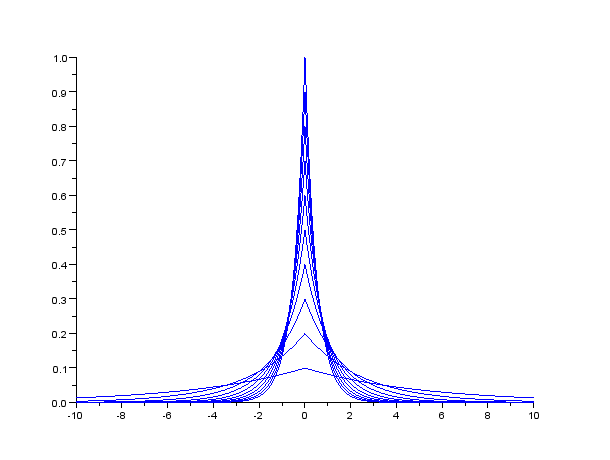
\includegraphics[scale=0.4]{Laplace.png}
\caption{Loi de l'erreur de Laplace en faisant varier le paramètre $m$ : plus il est élevé, plus l'erreur se disperse}
\label{fig:Laplace}
\end{figure}
  
On le voit, le raisonnement de Laplace l'amène à découvrir un cas où la moyenne arithmétique ne lui permet pas d'estimer correctement le paramètre $m$ ! Par manque de chance, il découvre une des exceptions que tout statisticien se doit de connaître aujourd'hui ! ( Le lecteur attentif aura bien sûr reconnu la loi de Laplace...)\\

C'est Gauss qui va renverser ce raisonnement, ce que l'on verra dans le paragraphe suivant : plutôt que de dériver une loi des erreurs d'après des hypothèses acceptables et de montrer qu'alors la moyenne empirique augmente la précision, il part de l'hypothèse que la moyenne empirique est la bonne chose à faire, et trouve la loi qui fait que cela fonctionne !

\subsection{Theoria Motus Corporum Coelestium in Sectionibus Conicis Solum Ambientium, Gauss 1809}

Cet article de Gauss, bien que traitant principalement des orbites des planètes, est fondamental dans le développement des statistiques mathématiques. C'est à ce moment qu'est réconciliée la méthode de combinaisons des observations formalisée par Legendre avec une approche probabiliste explicite : Gauss étudie un système linéaire à $\mu$ équations et à $\nu$ inconnues $p,q,r.,..$, dont on observe les coefficients $a,b,c,...$ :

\begin{align*}
V & = ap+bq+cr+...\\
V' & = a'p+b'q+c'r+...\\
V'' & = a''p+b''q+c''r+...\\
etc.
\end{align*}

Maintenant, et c'est l'étape cruciale, Gauss fait une hypothèse sur la loi des erreurs qu'il note $\Delta=V-M$, $\Delta'=V'-M'$,... : ces erreurs suivent toute la même loi donnée par la courbe $\phi$, et sont indépendantes. Cela lui permet de reformuler le problème : les coefficients $p,q,r,...$ maximisent la courbe d'événement :

\[\Omega = \phi(\Delta)\phi(\Delta')\phi(\Delta'')...\]

Les valeurs recherchées, note Gauss, peuvent se trouver en dérivant par rapport à $p,q,r,...$, à condition de posséder une expression exacte de la loi $\phi$. C'est ici la seconde étape importante de l'article où Gauss se démarque de Laplace.\\

Voici comment il dérive la loi des erreurs :  sa manière de les penser (les erreurs doivent se compenser) lui fait supposer que $\phi$ est maximale en $\Delta=0$ et symmétrique.  En d'autres termes, Gauss se simplifie la vie : plutôt que de chercher à justifier le principe de compensation des erreurs, il trouve directement une loi qui en est solution. Cela revient à inverser le problème par rapport à Laplace, en posant comme axiome que la valeur la plus probable issue d'observations répétées est la moyenne arithmétique.\\

Sous ces hypothèses, prendre
\[p=\frac{1}{\mu}(M+M'+M''+ ...)\]
maximise $\Omega$ seulement si 
\[\phi(\Delta)= \frac{h}{\sqrt \pi} e^{-h^2\Delta^2},\]
pour une certaine constante $h$ qui mesure la précision des observations. La preuve suivante est inspirée de celle de Gauss, avec des outils et des notations modernes.\\

La loi de probabilité des erreurs 
\[P(\Delta \in [\epsilon_1-\alpha;\epsilon_1+\alpha],\Delta' \in [\epsilon_2-\alpha;\epsilon_2+\alpha],\Delta'' \in [\epsilon_3-\alpha;\epsilon_3+\alpha])\]
vaut, par indépendance :
\[\prod_{i=1}^n \int_{\epsilon_i-\alpha}^{\epsilon_i+\alpha} \phi \sim (2\alpha)^n \prod \phi (\Delta^{(i)}).\]

Le changement de fonction inconnue $\psi =\log \phi$ nous amène à chercher une fonction $\psi$ telle que :
\[\Delta+\Delta'+\Delta''=0 \quad \Rightarrow \quad \psi(M-\Delta)+\psi(M-\Delta')+\psi(M-\Delta'') \text{ soit maximale en } M=0\]
c'est-à-dire à rechercher les fonctions $\phi$ vérifiant :
\[\Delta+\Delta'+\Delta''=0 \quad \Rightarrow \quad \psi'(\epsilon_1)+\psi'(\epsilon_2)+\psi'(\epsilon_3)=0.\]

Mais $\xi:= \psi'=\frac{\phi'}{\phi}$ est paire puisque $\phi$ l'est. Elle vérifie donc l'équation fonctionnelle :

\[\forall x,y\geq 0,  \xi(x+y)=\xi(x)+\xi(y),\]
dont les seules solutions continues  sont les fonctions linéaires $x\mapsto hx$. Notre brave fonction $\phi$ est donc solution de l'équation différentielle linéaire :
\[\frac{\phi'}{\phi}=hx.\]
l'unique solution d'intégrale $1$ sur $\R$ est alors :
\[\phi(\Delta)= \frac{h}{\sqrt \pi} e^{-h^2\Delta^2}.\]

\begin{figure}[!h]\centering
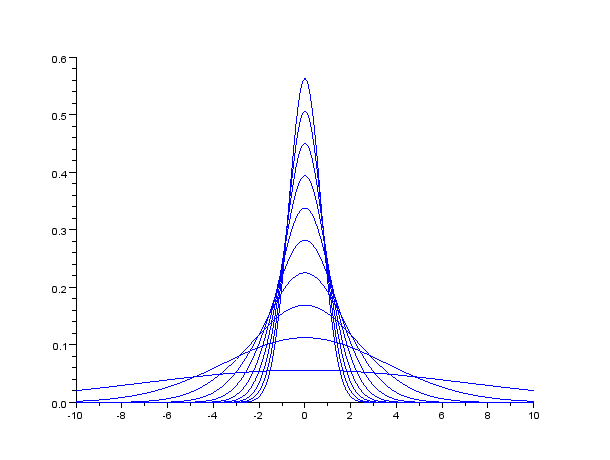
\includegraphics[scale=0.4]{Gaussienne.png}
\caption{Loi de l'erreur gaussienne en faisant varier le paramètre $h$ : plus il est élevé, plus l'erreur se disperse}
\label{fig:Gaussienne}
\end{figure}

\subsection{Vers le théorème de la limite centrale}

C'est donc Laplace, qui le premier, cherche à minimiser ce qu'il appelle l'erreur à craindre $\int |\Delta|\phi(\Delta)d\Delta$. A ce propos, il écrit :
\begin{quotation}
"Lorsque les observations sont en petit nombre, le choix de ces systèmes dépend de la loi des erreurs de chaque observation. Mais, si l'on considère un grand nombre d'observations, ... ce choix devient indépendant de cette loi et... l'Analyse conduit alors directement aux résultats de cette méthode des moindres carrés."
\end{quotation}

Laplace a ici une intuition : la loi des erreurs additionnées lorsque leur nombre est grand ne dépend pas des erreurs ; c'est le théorème central limite, démontré par Laplace après $1810$, et dont la première démonstration que l'on peut considérer comme rigoureuse a été donnée par Tchebycev en $1887$.\\

Gauss change la donne en cherchant à minimiser non plus $\int |\Delta|\phi(\Delta)d\Delta$ mais $\int \Delta^2 \phi(\Delta)d\Delta$. Avec le recul, le changement est seulement celui de la fonction d'erreur ou de perte : on passe du cadre $\mathcal L^1$ au cadre $\mathcal L^2$, qui est euclidien. Il semble que Gauss ait été influencé par la lecture de Laplace lorsqu'il publie \textit{Théorie de la Combinaison des Observations qui expose aux moindres erreurs}. Il y abandonne le point de vue "métaphysique" \cite{Chabert} et assoit définitivement la méthode des moindres carrés sur des méthodes probabilistes.\\

A ce moment s'opère une formalisation complète : les erreurs, lorsqu'on les somme, se compensent, et, si l'on peut les supposer gaussiennes dès le départ, c'est qu'une somme de variables aléatoires indépendantes, et de même loi, s'approche bien par une gaussienne. 

\subsection{Lecture commentée de l'article de 1816}

Le paragraphe qui suit est destiné à être une aide de lecture de certains passages de l'article original de Gauss : il est donc écrit en imagiant le lecteur suivant ledis %orthographe ?% 
 article en parallèle. J'ai gardé les notations de l'époque quand elles n'étaient pas trop lourdes. Par exemple, $h^2$ s'écrit $hh$, et l'erreur est notée $\Delta$ comme Gauss lui-même le fait.

\subsubsection{Introduction} Gauss commence son article en défendant l'intérêt de la constante $h$ dans la forme de la loi d'erreur :
\[\frac{h}{\sqrt \pi}e^{-hh\Delta\Delta},\]
forme obtenue dans son article de $1809$ où figure sa première preuve des MCO. %à vérifier
Pour lui, $h$ est une mesure de la précision, ce qui est conforme à l'écriture moderne que l'on peut en donner : $h=\frac{1}{\sigma\sqrt 2}$, où $\sigma$ est l'écart type. Sans référence à Bessel, qui introduit le terme d'\textit{erreur probable} en 1815, Gauss définit ensuite un paramètre $r$ comme la solution de :
\[\int_{-r}^r \frac{h}{\sqrt \pi}e^{-hh\Delta\Delta}d\Delta\] i.e. $r$ est le quantile de la loi normale $r=\Phi^{-1}(0,75)$, ainsi que $\rho=rh=0,4769363$.

\subsubsection{Estimation de $r$ et $h$ par la méthode des probabilités inverses.} Gauss commence par faire référence à son \textit{Theoria motus corporum coelestium} de $1809$, puis utilise une argument que l'on pourrait qualifier de Bayésien (méthode appelée à l'époque \textit{des probabilités inverses}) sans faire toutefois référence à Bayes, et qui lui sert à montrer que la densité \textit{a posteriori} est proportionnelle à la vraisemblance :
\[f(h|x)\propto f(x|h),\]
où il prend $h$ comme distribué de manière uniforme sur $[0,\infty)$. Bien que Laplace ait popularisé cette méthode en $1774$, Gauss ne le mentionne pas.\\
En maximisant $f(h|x)$ par rapportà $h$ Gauss obtient ce qu'Edwards avait appelé en $1974$ %verfier la date
l'estimateur \textit{le plus probable} :
\[\hat h = \left(\frac{m}{2\sum x_i^2}\right)^{\frac{1}{2}} \quad \text{où $m$ est la taille de l'échantillon}\]
\[\text{dont il déduit} \quad \hat r =\frac{\rho}{\hat h}\]

Une remarque importante : n'importe quel statisticien moderne reconnaît en $\hat h$ l'estimateur du maximum de vraisemblance, pourtant la différence de méthode est conceptuellement importante.\\

Gauss remarque que ce résultat est valable quel que soit la taille de l'échantillon $m$, mais il se place quand même dans un cadre asymptotique : $m$ est très grand, est alors la véritable valeur de $h$ est avec probabilité $\frac{1}{2}$ dans l'intervalle $(\hat h (1-\rho m^{\frac{1}{2}}),\hat h (1+\rho m^{\frac{1}{2}}))$. 
%%%%%%%%%%%%%%%%%%%%%%%%%%%%%%%%%%%%%%%%%%%%%%%%%%%%%%%%%%%%%%%%%%%%%%%%%%%%%%%%%%%%%%%%%
%%%%%%%%%%%%%%%%%%%%%%%%%%%%%%%%%%%%%%%%%%%%%%%%%%%%%%%%%%%%%%%%%%%%%%%%%%%%%%%%%%%%%%%%%
\section{Controverse sur le paradigme gaussien}

\subsection{Le modèle de Bachelier}

L'évaluation modernes des actifs financiers peut être datée, si tant est que cela soit possible, de la thèse de Louis Bachelier. De sa vie, on ne sait pas grand-chose, la plupart des archives le concernant ont été détruites. Né en 1870 et mort en 1946, il postule à un poste universitaire à Dijon, mais une mauvaise recommandation de Paul Lévy suite à une erreur dans l'une de ses publications le fait <<blackboulé>> ( Paul Lévy). Sa thèse, \textit{Théorie de la spéculation}, est loin d'être habituelle pour l'époque, ce qui contribuera à ralentir sa carrière. Il la soutient le 29 mars 1900, devant Henri Poincaré, rapporteur, qui écrira :
\begin{quotation}"Le sujet s'éloigne un peu de ceux qui sont habituellment traités par nos candidats" (Poincaré)\end{quotation}
Son travail est pourtant révolutionnaire, et beaucoup d'auteurs s'accordent à en reconnaître la modernité. Il s'intéresse à la prévision des cours boursiers. Pour cela, il remarque que des <<facteurs innombrables>> influent sur son comportement, dont il distingue ceux qui sont <<factices>> de ceux qui sont <<naturels>>. Plutôt que de prévoir exactement les prix futurs, il développe une approche probabiliste totalement novatrice : ces facteurs sont des accumulations de petits aléas, de petits chocs. Son idée est alors d'utiliser le seul outil dont il dispose à l'époque pour traiter les sommes de variables aléatoires, ou l'accumulation des erreurs : la loi normale. Ce n'est pas la seule hypothèse moderne que l'on retrouve dans son travail : il suppose que la spéculation est un jeu à somme nulle, en ses propres termes : 

\begin{quotation}
"On peut considérer deux sortes de probabilités. 1. La probabilité que l'on pourrait appeler mathématique
c'est celle que 'on peut déterminer a priori celle que on étudie dans les
jeux de hasard. 2. La probabilité dépendant de faits venir et par
conséquent impossible prévoir de fa on mathématique est cette der
nière probabilité que cherche prévoir le spéculateur il analyse les raisons
qui peuvent influer sur la hausse ou sur la baisse et sur amplitude des mou
vements Ses inductions sont absolument personnelles puisque sa contrepar
tie nécessairement opinion inverse" (Bachelier)
\end{quotation}
et la valeur future d'un cours ne dépend que de sa valeur présente, ce que l'on appelle aujourd'hui une martingale markovienne d'ordre $1$. Le problème qui nous intéresse ici est surtout celui de l'hypothèse de normalité des cours, puisque l'on verra dans la partie suivante que le problème de modélisation d'une multitude de chocs, ou de loi d'erreur, va subir une remise en question via l'introduction des lois stables par Paul Lévy.\\
 
\subsection{Paul Lévy}

Nous avons vu dans la première section de ce rapport que le cadre dans lequel baigne naturellement la Statistique Mathématique est gaussien. La loi de Gauss est considérée comme naturelle grâce au théorème central-limite qui assure que la somme cumulée des erreurs, renormalisée, se comporte asymptotiquement comme une normale.\\

Résumons en quelques mots l'histoire que nous avons raconté dans la seconde partie de ce rapport. Gauss effectue la première régression linéaire, si l'on en croit ses dires, afin de repérer le premier astéroïde jamais observé, Cérès, et cette méthode est formalisée par Legendre quelques années plus tard, puis par Gauss, qui en donne une démonstration plus complète. Cette méthode est basée sur une vieille "recette de cuisine", la méthode des milieux, qui est déjà utilisée depuis longtemps en navigation et en géodésie.\\

 Arrive Laplace, qui souhaite effectivement montrer que prendre la moyenne arithmétique des observations augmente la précision d'une mesure grâce à un calcul effectif d'analyse mathématique. Toutefois, il se heurte à un problème : mener le calcul à son terme nécessite de choisir une loi précise, or il refuse les lois rectangulaires ou triangulaires de ses contemporains. Il se sert donc d'un de ses principes préférés, celui de raison insuffisante, afin de dériver une loi à partir d'hypothèse qu'il peut accepter. Ses calculs, par malchance, le mènent à la loi de Laplace (nommée ainsi plus tard), dont un estimateur du premier moment est plutôt la médiane empirique. En tout cas, la moyenne ne fonctionne pas dans ce cas là.\\

 Inspiré par Laplace, Gauss inverse le problème en supposant que prendre la moyenne est bien ce qu'il faut faire. Il en déduit la loi normale par un calcul et des restrictions sur le type de loi qu'il s'autorise. Laplace, raffinant un théorème d'un Bernoulli, arrive à une "démonstration" du théorème de la limite centrale. La boucle est bouclée : les erreurs de mesure, si on les moyenne, suivent approximativement une loi normale, ce qui permet d'asseoir la méthode des moindres carrés sur des bases théoriques solides.\\

Toutefois, une lecture attentive du théorème révèle quelques hypothèses techniques : les erreurs que l'on somme sont des réalisations de variables aléatoires indépendantes et identiquement distribuées, qui ont une espérance et une variance. Qu'en est-il lorsque la variance est infinie ? Cette question ne sera pas soulevé pendant assez longtemps, et je n'en ai pas trouvé de trace avant le traitement qu'en a fait Paul Lévy au XIXè siècle.\\

Paul Lévy est un mathématicien né en 1886, il a fait Polytechnique et le Corps des Mines. Il a entre autres %vérifier l'orthographe%
été le professeur de Benoît Mandelbrot et de Laurent Schwartz (qui était aussi son gendre), ce qui aura son importance comme nous le verrons : Benoît Mandelbrot le cite souvent en exemple lorsqu'il critique violement les modèles économiques actuels. Paul Lévy est un précurseur en analyse fonctionnelle, où il suit les travaux de Volterra sur les "équations de lignes", c'est à dire les fonctionnelles (fonctions qui prennent en argument des fonctions) puis il est un des premiers à étudier et à fonder la théorie des probabilités sur des bases modernes. Précisons qu'il ne participe pas à la formulation $(\Omega,A,\mathbb P)$ des probabilités que l'on enseigne aujourd'hui, liée à Kolmogorov. A ce propos, Laurent Scwartz a écrit :

\begin{quotation}
"Je n'ai jamais vraiment compris à cette époque, du point de vue mathématique, ce qu'étaient des variables aléatoires et il [Paul Lévy] n'a jamais pu me l'expliquer. Il me l'expliquait comme un physicien ; les variables aléatoires sont indépendantes si elles correspondent à des tirages au sort dont chacun ignore le résultat des autres, il s'agit là d'une définition physique ; assez rapidement on arrive à en tirer un certain nombre de déductions qui s'écrivent très bien sous forme mathématique, par exemple le fait que la probabilité de réalisation de deux événements simultanés indépendants est le produit des probabilités de ces événements ; on pouvait écrire aussi cela avec la notion de probabilités conditionnelles ; mais tout cela restait extrêmement flou et fort difficile à comprendre en profondeur sur le plan des mathématiques, telles que nous les envisageons aujourd'hui.\\
Je ne crois d'ailleurs pas que Paul LÉVY aurait pu s'arrêter à une axiomatique rigoureuse du calcul des probabilités. Tout était encore à faire dans ce domaine ; il aurait dû pratiquement y passer des années dans son existence, et ce n'était visiblement pas cela qui l'intéressait le plus." (Laurent Schwartz, \url{ http://www.annales.org/archives/x/paullevy.html} )
\end{quotation}

Les travaux des P. Lévy sont très intéressants, et nous renvoyons le lecteur intéressé au lien dans la citation, qui contient de nombreux témoignages. Nous ne pouvons pas résister à signaler que c'est lui qui semble avoir été à l'origine de l'introduction de la fonction de répartition lorsque l'on traite d'une variable aléatoire, réunissant ainsi les cadres discrets et continus, ce qui est une méthode que l'auteur trouve esthétique. Il est aussi un pionnier en ce qui concerne les modes de convergence de variables aléatoires. La plupart des déclarations de ce rapport concernant P. Lévy ont son livre \textit{Quelques aspects de la pensée d'un mathématicien} comme source.\\

P. Lévy s'intéresse aux probabilités après avoir été chargé d'en donner des cours à l'école Polytechnique à la suite de Henri Poincaré, qui n'était pas satisfait de la rédaction qu'il en avait donné. Il s'intéresse vite à "la loi de Gauss", comme on peut le lire :

\begin{quotation}
"Pour la théorie des erreurs, je me rappelais seulement que les erreurs accidentelles obéissent à la loi de Gauss, et que c'était dû à ce qu'elles résultent de diverses causes indépendantes, dont chacune a un effet négligeable." (Paul Lévy, Quelques aspects de la pensée d'un mathématicien)\\
\end{quotation}

\begin{quotation}
"Deux ou trois ans plus tard, quand nous étions élèves à l'École des Mines, mon camarade et ami Belugou me dit un jour: <<Je 
viens de lire le calcul des prohahilités de Borel ; il y a une admirable démonstration de la loi de Gauss. >> Intrigué, je lus cette démonstration. Il s'agissait du calcul asymptotique dû à de Moivre, par lequel on établit le rôle de la loi de Gauss dans le cas de Bernoulli. C'est, comme l'on sait, un très joli calcul, mettant en évidence le fait qu'après une réduction convenable la courbe des coefficients du binôme de Newton, pour un exposant indéfiniment croissant, tend vers celIe de Gauss. Je ne le connaissais pas, mais j'avais trop souvent fait des calculs analogues pour m'étonner de celui-là. Par contre, il me parut évident qu'on ne pouvait pas considérer l'étude d'un cas si particulier, qui ne saurait être réalisé en pratique, comme une explication de la loi de Gauss relative aux erreurs d'observation. Comment Borel 
a-t-il pu s'en contenter ?" (Paul Lévy, Quelques aspects de la pensée d'un mathématicien ~\cite{Lévy}) \\
\end{quotation}

Il donnera une des premières preuves modernes du théorème de la limite centrale. En parallèle, il introduit les lois stables à la suite d'une discussion avec le capitaine Lhoste, qui lui affirme à tort que la loi de Gauss est la seule loi stable. Par stable, on entend une loi telle que si $X_1$ et $X_2$ en sont deux réalisations indépendantes, et $a_1$ et $a_2$ deux constantes positives, alors $a_1X_1+a_2X_2 $ est de la forme $aX$, où $X$ suit cette même loi,et $a>0$. En refléchissant, Lévy comprend que tout variable aléatoire dont la fonction de répartition est de la forme $e^{c|z|^{\alpha}}$ est stable. (Bien entendu, $0<\alpha\leq2$.) Pour $\alpha=2$, on retrouve la loi normale, et si $\alpha=1$, on obtient la loi de Cauchy :
\[P(X\leq x)=\int_{-\infty}^x \frac{du}{\pi(u^2+1)}.\]

La notion de stabilité et sa démonstration du théorème central-limite grâce aux fonctions caractéristiques lui permettent de généraliser ce dernier. Voici comment. On dit qu'une suite de variables aléatoires est dans le domaine d'attraction d'une loi $G$ s'il existe des suites $a_n$ et $b_n$ telles que :
\[\frac{X_1+X_2+...+X_n-a_n}{b_n}\]
converge en loi vers la loi $G$. Alors, si les variables aléatoires ont essentielement des moments d'ordre un et deux, on retrouve le théorème de <<la loi de Gauss>> habituel. Toutefois, sous des conditions plus faibles, on peut avoir convergence vers une loi stable. Le paragraphe suivant donne l'énoncé précis du théorème.\\

On suppose que les erreurs $\epsilon_i$ obéissent à une loi dont la fonction de répartition vérifie :

\[1-F(x)\sim_{+\infty} x^{-\alpha}L(x)\quad\text{et}\quad F(-x)\sim_{+\infty}cx^{-\alpha} L(x)\]
pour un $\alpha \in [1;2]$, et $L:\R_+^*\rightarrow \R_+^*$ une fonction à variation lente au voisinage de $+\infty$.\\

 Si $1<\alpha<2$, alors $\mu=\int |x| dP<\infty$ mais $\int x^2 dP = \infty$. S'il existe deux suites $a_n$ et $b_n$ telles que $\left(\sum_{i=1}^n X_i -b_n\right)/a_n$ converge en loi vers la loi $\alpha$-stable, donnée par :
\[\int e^{itx}Q_\alpha(dx)=\left\{\begin{array}{lr}\exp(-\sigma^\alpha |t|^\alpha\left(1-i\beta sg(t)\tan(\frac{\pi\alpha}{2})\right)) & \text{si }\alpha\neq 1\\ 
\exp(-\sigma |t|\left(1-i\beta sg(t)\log|t|\right))& \text{si }\alpha=1\end{array}\right.,\]
 on dit que les erreurs sont dans le bassin d'attraction de la loi $\alpha$-stable $Q_\alpha$.\\

Paul Lévy a établi un analogue du théorème central limite : si $P$ est dans le bassin d'attraction de $Q_\alpha$ et que $1<\alpha\leq2$, alors la moyenne arithmétique est asymptotiquement $\alpha$-stable :
\[
\begin{tikzcd}[column sep = small]
n^{1-\frac{1}{\alpha}}\left(\sum_{i=1}^n \epsilon_i-\mu\right)\arrow{r}{\mathcal L} & Q_\alpha
\end{tikzcd}\]

\begin{figure}[!h]\centering
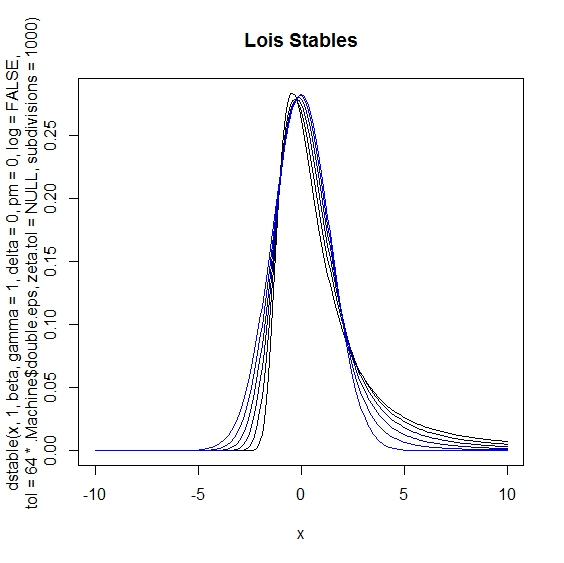
\includegraphics[scale=0.4]{Stables.jpeg}
\caption{Densité de lois stables. Plus la courbe est bleue, plus $\alpha$ se rapproche de $2$, et l'on retrouve la loi de Gauss.}
\label{fig:Stables}
\end{figure}

\subsection{Efficience des marchés}
% Si ce théorème est important, c'est qu'il va provoquer une remise en question de \\%%%%%%%%%

La thèse de Louis Bachelier provoque un changement de paradigme en finance. L'objet d'étude se déplace de la prévisibilité du cours à la volatilité du marché. Le but des analystes quantitatifs d'aujourd'hui n'est pas de prévoir la valeur futur du cours, mais bien d'en estimer la volatilité instantanée potentielle. Mieux, ils essaient d'estimer comment les cours varient deux à deux, au moyen de ce que l'on appelle la matrice de variance-covariance, afin d'optimiser le risque en trouvant la meileure la proportion de chaque actif du portefeuille.\\

Le modèle de Bachelier va être testé statistiquement, sur au moins deux points :
\begin{itemize}
\item l'absence de mémoire du marché, donc de prévisibilité. On teste dans ce cas l'indépendance des accroissements des cours.
\item l'hypothèse de variablité normale. On s'intéresse ici aux risques de changements de prix.\\
\end{itemize}

Les tests pratiqués semblent valider le modèle, successivement par Working (1934), Cowles et Jones (1937) et Kendall (1953), et mettent en évidence une absence d'autocorrélation entre les variations successives des prix. Osbourne introduit en 1959 ~\cite{Osbourne} un changement dans la modélisation en considérant les logarithmes des prix. En s'inspirant de principes de mécanique statistique, il utilise le mouvement brownien pour modéliser les cours de la même façon que des particules dans un gaz. Bien que Louis Bachelier ait eu l'intuition du mouvement brownien, il ne sera pas formulé mathématiquement avant les travaux de Norbert Wiener en 1923. En cela, Osbourne est le premier à introduire le mouvement brownien en un sens moderne en finance. D'autres travaux confirment alors que la variation des prix relatifs peut être modélisée par un mouvement brownien : Larsen (1960), Working (1960), Houthakker (1961),... Nous renvoyons à l'article de Walter pour plus de détails. La loi de variations des prix relatifs et l'indépendance des accroisssements du modèle de Bachelier ne semblent pas être dissociés à l'époque : Walter parle de vision <<Gauss-markovienne>> des marchés. Cette vision restera dominante à partir de ces validations empiriques, et ne bénéficiera d'aucune remise en question jusqu'au krach de 1987.\\

Ce paradigme <<statistique-probabiliste>> des marchés, pour reprendre les termes de Walter, va être accentué par le développement parallèle de la théorie de gestion des protefeuilles. Harry Markovitz propose en 1952 ~\cite{Markowitz} un nouvelle méthode : maximiser la rentabilité sous la contrainte d'un risque fixé, ou le problème dual, minimiser le risque en fixant la rentabilité. La théorie moderne du portefeuille, qui en découle, emergera dans les années 60 grâce aux simplifications des calculs, obtenus par Sharpe en 1963 ~\cite{Sharpe}. Cette théorie, celle de la matrice de variance-covariance, permet de calculer effectivement les portefeuilles optimaux de Markovitz, moyennant une <<hypothèse économique audacieuse>> (Walter ~\cite{Walter}). Cette technologie, mise à disposition des société de gestion, utilise implicitement le modèle de Bachelier-Osbourne, et donc les hypothèses économiques sous-jacentes, en particulier celle de multi-normalité des actifs (on suppose que chaque titre suit une loi normale, dont les relations d'indépendance sont entièrement données par la matrice de variance-covariance). Ce dogme <<Gauss-markovien>> va être définitivement érigé comme axiome financier avec l'apparition de la théorie des options. L'hypothèse gaussienne sera tellement importante dans les modèles, qui utilisent des processus de diffusions et suppose donc des variances finies, qu'elle ne pourra pas être remise en cause. Ici encore, soulignons l'avance de Bachelier. En cherchant à calculer la probabilité qu'un titre atteigne ou dépasse une valeur donnée en une durée determinée, il réussit à retrouver le noyau de la chaleur, ce qui l'amène à établir un analogie entre les prix et la théorie analytique de la chaleur. Bachelier avait donc exhibé à l'époque le lien entre équation de la chaleur et mouvement brownien ! C'est ce lien qui sera exploité soixante-dix ans plus tard lorsque Black et Scholes utiliseront l'équation de la chaleur pour évaluer des options. Voici ce qu'en dit Poincaré :\\

\begin{quotation}
"La manière dont Louis Bachelier tire la loi de Gauss est fort originale et d'autant plus intéressante que le raisonnement pourrait s'étendre avec quelques changements à la théorie des erreurs. Il le développe dans un chapitre dont le titre peut abord sembler étrange car il l'intitule <<Rayonnement de la probabilité>>. C'est en effet à une comparaison avec la théorie analytique de la propagation de la chaleur que l'auteur a eu recours. Un peu de réflexion montre que l'analogie est réelle et la comparaison légitime. Les raisonnements de Fourier sont applicables presque sans changements à ce problème si différent de celui pour lequel ils ont été créés. On peut regretter que l'auteur n'ait pas développé davantage cette partie de sa thèse." (Henri Poincaré, Rapport de la thèse de Bachelier)
\end{quotation}

Avec la naissance de la théorie des options, fondée sur la théorie des processus de diffusions gaussiens, la technologie financière devient dépendante du modèle de Bachelier-Osbourne. Seule l'hypothèse de normalité de la volatilité du marché permet les calculs effectifs qui permettent aux sociétés de couvrir une position.\\

%Controverse analystes%
Si les économistes universitaires soutiennent le modèle Gauss-markovien, les analystes techniques essaient quant à eux de prévoir les <<tendances>> du marchés. Les \textit{chartists} par exemple examinent les graphiques d'évolution des cours en essayant d'y discerner des motifs récurents. Ils espèrents ainsi récupérer une information avant les autres, et pouvoir en tirer profit. Cette technique est en contradiction flagrante avec les théories universitaires, ce qui provoquera une polémique, celle des <<analystes techniques>>. Les universitaires y voient une sorte de numérologie moderne face à un phénomène imprévisible, alors que les analystes repochent aux universitaires d'être perdus dans leurs constructions intellectuelles, sans aucun lien avec la réalité. Cette controverse atteindra un <<\textit{statu quo} temporaire>> avec l'analyse que propose Cootner. \\

En 1965, Fama ~\cite{Fama} publie un article dans lequel il affirme que, sur les études statistiques qu'il a menées, il ne trouvait pas de résultats significatifs d'interdépendance. Son interprétation est que, bien que le marché présente une sorte de <<mémoire à court terme>>, ce non équilibre local n'invalide pas l'hypothèse de marche au hasard. Notons que, des techniques statistiques disponibles plus tard montreront que le marché peut subir des effets à long terme, et donc posséder une <<mémoire longue voir infinie>>.\\

La controverse commence avec la publication par Mandelbrot en $1962$ d'un modèle qui propose de modéliser les accroissements des log-rendements par des processus de Lévy (les accroisements sont des lois stables). Les innombrables chocs opérant sur les marchés boursiers ne sont plus de carré intégrable ! Les chocs ne sont plus <<homogènes et de même nature>>, mais <<hétérogènes et fortement hierarchisés>> ~\cite{Walter}. L'utilisation de variables à queues épaisses apporte une idée nouvelle vis à vis des événements rares : certains chocs ont une importance démesurée par rapport au reste de l'échantillon. Pour reprendre un exemple de \textit{Les cygnes noirs} de Taleb, la différence entre le hasard des lois normales, et celui des lois à queues épaisses peut s'illutrer ainsi. Si vous réunissez $1000$ personnes au hasard, et que vous observez la distribution de la taille dans l'échantillon, vous ne serez guère surpris. En effet, peut importe la plus grande personne que vous puissiez imaginer, sa taille ne déviera pas beaucoup de la moyenne. Par contre, relevez le revenu de chacun. Il est fort probable que une petite fraction des plus riches concentrent la majorité de la valeur. Si par malchance vous avez tiré dans votre échantillon un Bill Gates, son revenu constituera sans doute plus de $99\%$ de la valeur totale. C'est en ce sens que Mandelbrot propose des lois au hasard plus <<sauvage>>, qu'il nomme hasard de Pareto. Un événement rare peut décider de l'issue du marché. Voici ce qu'il écrit :

\begin{quotation}

Les chroniques boursières sont telles que l'on aucun espoir de pouvoir leur appliquer le modèle le plus simple, et par conséquent le plus tentant, de fluctuation régie par le hasard, à savoir le mouvement brownien, qui postule que les changements successifs des prix sont des variables aléatoires gaussiennes indépendantes
Comme une prédiction boursière non probabiliste est notoirement impossible il faut modifier le mouvement brownien.
\end{quotation}

Faute de techniques statistiques adaptées au moment des publications des différents modèles proposés par Mandelbrot, la controverse se finiera par un statu-quo entre la MV-efficience et le hasard de Pareto. En effet, l'abandon de fluctuations de carré intégrable force les statisticiens à inventer de nouvelles méthodes, ce qui prend du temps (et de l'argent). Aussi, il faudra attendre le krach de $1987$ pour que soit remis en cause le concept d'efficience. Pour plus de détails, nous renvoyons à l'excellent article de Walter ~\cite{Walter}. Bien que l'auteur aurait aimé aller plus loin, le manque de temps lui fait clore ici ce rapport.\\

%%%%%%%%%%%%%%%%%%%%%%%%%%%%%%%%%%%%%%%%%%%%%%%
%%%%%%%%%%%%%%%%%%%%%%%%%%%%%%%%%%%%%%%%%%%%%%%

%\subsection{Méthode directe.}
%\section{Entropie}
%Entropie en physique.\\
%démonstration du TCL avec l'entropie.
\bibliographystyle{plain}
\bibliography{Histoire}
\nocite{*}


\end{document}


























